% fig_ibr_voltage_profile.tex
% TR-29: |V_relay| vs fault location alpha for SG and IBR sources
%
% V_relay(SG)  = V_pre * alpha * Z_line / (Z_src + alpha * Z_line)
%              = 1.0  * alpha * 0.05 / (0.10 + 0.05*alpha)
% V_relay(IBR) = k_ibr * alpha * Z_line = k_ibr * alpha * 0.05
%
% Reference thresholds:
%   V_min_self   = 0.10 pu  (self-polarised Mho minimum)
%   V_min_memory = 0.02 pu  (memory / cross-pol minimum)
%
% Key finding:
%   SG V_relay: 0.048 pu at alpha=0.10, rising to 0.333 pu at alpha=1.0
%   IBR max V_relay (k=0.20, alpha=1.0): 0.010 pu — always below V_min_self
%   => ALL IBR-fed line faults on this network require cross-polarisation

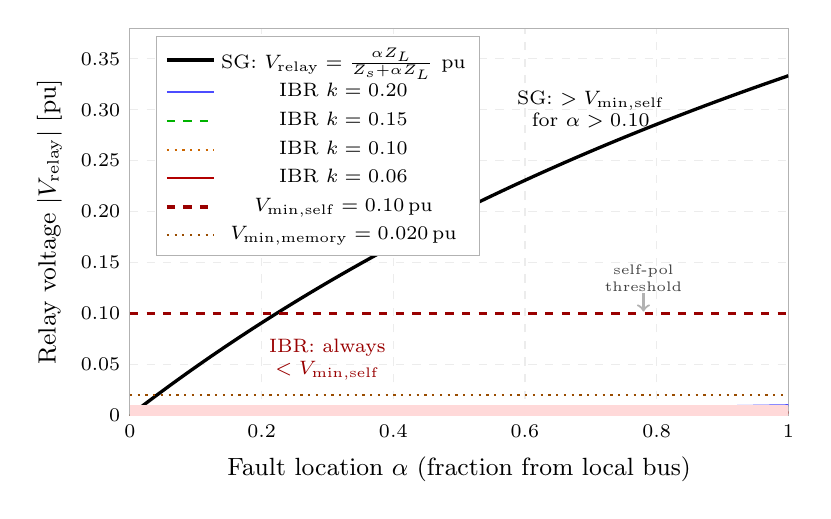
\begin{tikzpicture}
\begin{axis}[
  name         = voltax,
  width        = 0.82\textwidth,
  height       = 6.5cm,
  xlabel       = {Fault location $\alpha$ (fraction from local bus)},
  ylabel       = {Relay voltage $|V_{\rm relay}|$ [pu]},
  xlabel style = {font=\small},
  ylabel style = {font=\small},
  xmin=0, xmax=1.0,
  ymin=0, ymax=0.38,
  xtick        = {0, 0.2, 0.4, 0.6, 0.8, 1.0},
  xticklabel style={font=\scriptsize},
  ytick        = {0, 0.05, 0.10, 0.15, 0.20, 0.25, 0.30, 0.35},
  yticklabels  = {0, 0.05, 0.10, 0.15, 0.20, 0.25, 0.30, 0.35},
  yticklabel style={font=\scriptsize},
  legend style={at={(0.04,0.98)}, anchor=north west,
                font=\scriptsize, draw=gray!60},
  grid         = major,
  grid style   = {gray!15, dashed},
  tick style   = {draw=none},
  axis line style={gray!60},
]

% SG voltage profile (from analytical formula)
\addplot[black, very thick, domain=0.01:1.0, samples=80]
  ({x}, {x * 0.05 / (0.10 + x * 0.05)});
\addlegendentry{SG: $V_{\rm relay}=\frac{\alpha Z_L}{Z_s+\alpha Z_L}$ pu}

% IBR k=0.20
\addplot[blue!70, thick, domain=0:1.0, samples=2]
  ({x}, {0.20 * x * 0.05});
\addlegendentry{IBR $k=0.20$}

% IBR k=0.15
\addplot[green!70!black, thick, dashed, domain=0:1.0, samples=2]
  ({x}, {0.15 * x * 0.05});
\addlegendentry{IBR $k=0.15$}

% IBR k=0.10
\addplot[orange!80!black, thick, dotted, domain=0:1.0, samples=2]
  ({x}, {0.10 * x * 0.05});
\addlegendentry{IBR $k=0.10$}

% IBR k=0.06
\addplot[red!70!black, thick, domain=0:1.0, samples=2]
  ({x}, {0.06 * x * 0.05});
\addlegendentry{IBR $k=0.06$}

% Threshold lines
\addplot[red!60!black, very thick, dashed, mark=none, domain=0:1.0, samples=2]
  ({x}, {0.10});
\addlegendentry{$V_{\rm min,self}=0.10$\,pu}

\addplot[orange!60!black, thick, dotted, mark=none, domain=0:1.0, samples=2]
  ({x}, {0.020});
\addlegendentry{$V_{\rm min,memory}=0.020$\,pu}

% Shaded band: IBR maximum (0-0.010 pu) vs self-pol threshold
\addplot[red!15, fill, draw=none, domain=0:1.0, samples=2]
  coordinates {(0, 0) (1.0, 0) (1.0, 0.010) (0, 0.010)};


% Annotation: SG zone
\node[font=\scriptsize, black, align=center]
  at (axis cs:0.70, 0.30)
  {SG: $>V_{\rm min,self}$\\for $\alpha>0.10$};

% Annotation: IBR zone
\node[font=\scriptsize, red!60!black, align=center]
  at (axis cs:0.30, 0.055)
  {IBR: always\\$<V_{\rm min,self}$};

% Memory window annotation
\draw[->, gray!60, thick]
  (axis cs:0.78, 0.12) -- (axis cs:0.78, 0.102);
\node[font=\tiny, gray!50!black, align=center]
  at (axis cs:0.78, 0.135)
  {self-pol\\threshold};

\end{axis}
\end{tikzpicture}
